\DocumentMetadata{%
  lang = en-us,
  pdfversion = 2.0,
  pdfstandard = ua-2,
  tagging = on,
  tagging-setup = {math/setup=mathml-SE}
}
\tagpdfsetup{activate, tabsorder=structure}
% Options for packages loaded elsewhere
\PassOptionsToPackage{dvipsnames,svgnames,x11names}{xcolor}
%
\documentclass[
  letterpaper,
  DIV=11,
  numbers=noendperiod]{scrartcl}

\usepackage{xcolor}
\usepackage{fancyvrb}
\newcommand{\VerbBar}{|}
\newcommand{\VERB}{\Verb[commandchars=\\\{\}]}
\DefineVerbatimEnvironment{Highlighting}{Verbatim}{commandchars=\\\{\}}
% Add ',fontsize=\small' for more characters per line
\usepackage{framed}
\definecolor{shadecolor}{RGB}{241,243,245}
\newenvironment{Shaded}{\begin{snugshade}}{\end{snugshade}}
\newcommand{\BuiltInTok}[1]{\textcolor[rgb]{0.00,0.23,0.31}{#1}}
\newcommand{\ExtensionTok}[1]{\textcolor[rgb]{0.00,0.23,0.31}{#1}}
\newcommand{\NormalTok}[1]{\textcolor[rgb]{0.00,0.23,0.31}{#1}}

\providecommand{\tightlist}{%
  \setlength{\itemsep}{0pt}\setlength{\parskip}{0pt}}\usepackage{longtable,booktabs,array}
\usepackage{calc} % for calculating minipage widths
% Allow footnotes in longtable head/foot
\IfFileExists{footnotehyper.sty}{\usepackage{footnotehyper}}{\usepackage{footnote}} % there is an issue with this package and tagpdf - always generates warning on render
\makesavenoteenv{longtable}
\usepackage{graphicx}
\makeatletter
\newsavebox\pandoc@box
\newcommand*\pandocbounded[1]{% scales image to fit in text height/width
  \sbox\pandoc@box{#1}%
  \Gscale@div\@tempa{\textheight}{\dimexpr\ht\pandoc@box+\dp\pandoc@box\relax}%
  \Gscale@div\@tempb{\linewidth}{\wd\pandoc@box}%
  \ifdim\@tempb\p@<\@tempa\p@\let\@tempa\@tempb\fi% select the smaller of both
  \ifdim\@tempa\p@<\p@\scalebox{\@tempa}{\usebox\pandoc@box}%
  \else\usebox{\pandoc@box}%
  \fi%
}
% Set default figure placement to htbp
\def\fps@figure{htbp}
\makeatother

\KOMAoption{captions}{tableheading}
\makeatletter
\@ifpackageloaded{tcolorbox}{}{\usepackage[skins,breakable]{tcolorbox}}
\@ifpackageloaded{fontawesome5}{}{\usepackage{fontawesome5}}
\definecolor{quarto-callout-color}{HTML}{909090}
\definecolor{quarto-callout-note-color}{HTML}{0758E5}
\definecolor{quarto-callout-important-color}{HTML}{CC1914}
\definecolor{quarto-callout-warning-color}{HTML}{EB9113}
\definecolor{quarto-callout-tip-color}{HTML}{00A047}
\definecolor{quarto-callout-caution-color}{HTML}{FC5300}
\definecolor{quarto-callout-color-frame}{HTML}{acacac}
\definecolor{quarto-callout-note-color-frame}{HTML}{4582ec}
\definecolor{quarto-callout-important-color-frame}{HTML}{d9534f}
\definecolor{quarto-callout-warning-color-frame}{HTML}{f0ad4e}
\definecolor{quarto-callout-tip-color-frame}{HTML}{02b875}
\definecolor{quarto-callout-caution-color-frame}{HTML}{fd7e14}
\makeatother
\makeatletter
\@ifpackageloaded{caption}{}{\usepackage{caption}}
\AtBeginDocument{%
\ifdefined\contentsname
  \renewcommand*\contentsname{Table of contents}
\else
  \newcommand\contentsname{Table of contents}
\fi
\ifdefined\listfigurename
  \renewcommand*\listfigurename{List of Figures}
\else
  \newcommand\listfigurename{List of Figures}
\fi
\ifdefined\listtablename
  \renewcommand*\listtablename{List of Tables}
\else
  \newcommand\listtablename{List of Tables}
\fi
\ifdefined\figurename
  \renewcommand*\figurename{Figure}
\else
  \newcommand\figurename{Figure}
\fi
\ifdefined\tablename
  \renewcommand*\tablename{Table}
\else
  \newcommand\tablename{Table}
\fi
}
\@ifpackageloaded{float}{}{\usepackage{float}}
\floatstyle{ruled}
\@ifundefined{c@chapter}{\newfloat{codelisting}{h}{lop}}{\newfloat{codelisting}{h}{lop}[chapter]}
\floatname{codelisting}{Listing}
\newcommand*\listoflistings{\listof{codelisting}{List of Listings}}
\makeatother
\makeatletter
\makeatother
\makeatletter
\@ifpackageloaded{caption}{}{\usepackage{caption}}
\@ifpackageloaded{subcaption}{}{\usepackage{subcaption}}
\makeatother

\usepackage{bookmark}

\IfFileExists{xurl.sty}{\usepackage{xurl}}{} % add URL line breaks if available
\urlstyle{same} % disable monospaced font for URLs
\hypersetup{
  pdftitle={Quarto a11y feature testing},
  colorlinks=true,
  linkcolor={blue},
  filecolor={Maroon},
  citecolor={Blue},
  urlcolor={Blue},
  pdfcreator={LaTeX via pandoc}}


\title{Quarto a11y feature testing}
\author{}
\date{}

\begin{document}
\maketitle


\subsection{Making Quarto pdf more
accessible}\label{making-quarto-pdf-more-accessible}

Yaml pre-requisites:

\begin{itemize}
\tightlist
\item
  lualatex engine
\item
  full install of tinytex (bundle = ``TinyTeX-2'')
\item
  \texttt{keep-tex:\ true} to keep the tex file for debugging
\end{itemize}

\subsection{Rendering Figures}\label{rendering-figures}

The following figures are made within a quarto doc and get produced from
the R code chunks below. Their alternative text is stored in the
captions\_alt\_text.csv file.

The add\_alttext() function sourced from a11y\_script.R uses the
captions\_alt\_text.csv file to find and match the alt text to the
produced figures.

\begin{figure}

\centering{

\pandocbounded{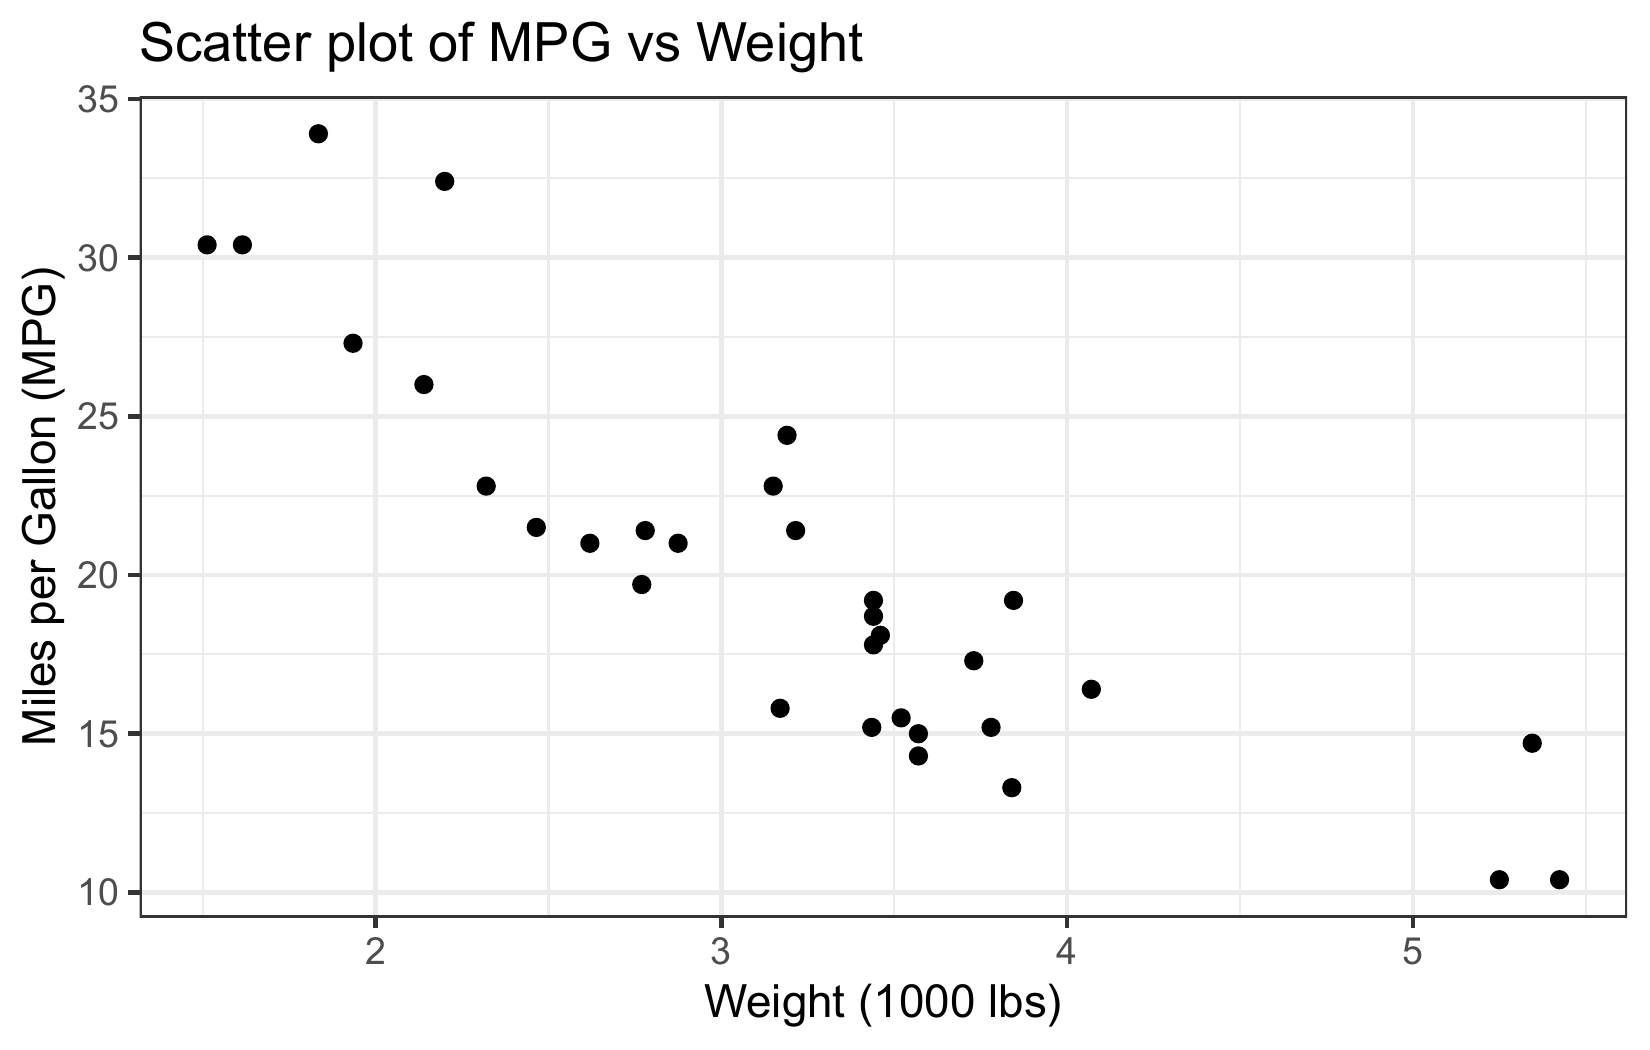
\includegraphics[keepaspectratio,alt={'A scatter plot of mile per gallon versus weight of cars with weight in 1000 pounds is on the x axis and miles per gallon is on the y-axis.'}]{quarto_a11y_files/figure-pdf/fig-cars-1.png}}

}

\caption{\label{fig-cars}A scatter plot of MPG vs Weight}

\end{figure}%

\begin{itemize}
\tightlist
\item
  Recommended: load image still from a chunk so it's easier to add
  options
\end{itemize}

\begin{figure}

\centering{

\pandocbounded{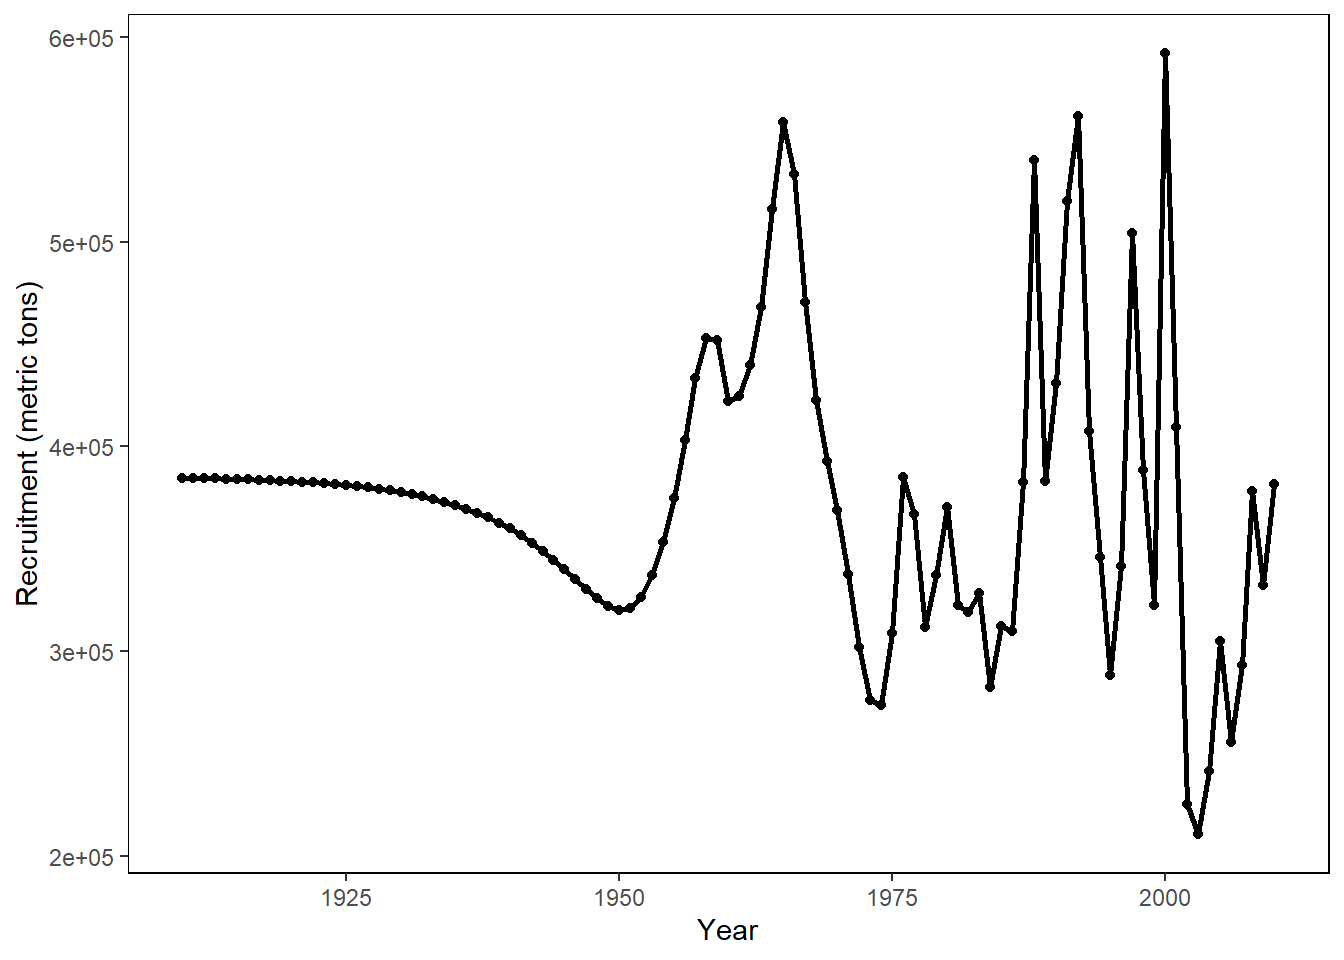
\includegraphics[keepaspectratio,alt={'Alternative text for an image loaded in an R chunk from knitr::include_graphics()'}]{figures/figure.png}}

}

\caption{\label{fig-random}This is the caption for the second plot.}

\end{figure}%

Ways to add alt text to figures in pdf from latex:

\emph{For non-chunk figures, user needs to specify the label for our
function to work}

\begin{itemize}
\tightlist
\item
  @ the end of the reference to figure line you can add brackets
  containing the alt text
\end{itemize}

\begin{Shaded}
\begin{Highlighting}[]
\NormalTok{![](figures/figure.png)\{alt="Here is my alt text for this image",\#fig{-}testa\}}
\end{Highlighting}
\end{Shaded}

\begin{itemize}
\tightlist
\item
  within the brackets specifting alt=``text'' (this method is not
  working though)
\end{itemize}

\begin{Shaded}
\begin{Highlighting}[]
\NormalTok{![alt=This is my alternative text for this image](figures/figure.png)\{\#fig{-}testb\}}
\end{Highlighting}
\end{Shaded}

\subsubsection{How it's done in latex}\label{how-its-done-in-latex}

\begin{Shaded}
\begin{Highlighting}[]
\BuiltInTok{\textbackslash{}includegraphics}\NormalTok{[keepaspectratio,alt=\{"This is alt text"\}]\{}\ExtensionTok{figures/figure.png}\NormalTok{\}}
\end{Highlighting}
\end{Shaded}

\begin{tcolorbox}[enhanced jigsaw, coltitle=black, title=\textcolor{quarto-callout-note-color}{\faInfo}\hspace{0.5em}{Note}, titlerule=0mm, left=2mm, opacitybacktitle=0.6, colframe=quarto-callout-note-color-frame, bottomrule=.15mm, breakable, colback=white, colbacktitle=quarto-callout-note-color!10!white, opacityback=0, arc=.35mm, leftrule=.75mm, bottomtitle=1mm, toptitle=1mm, rightrule=.15mm, toprule=.15mm]

The above method is the recommended practice and what is used in our
add\_alttext() function

\end{tcolorbox}

\begin{Shaded}
\begin{Highlighting}[]
\BuiltInTok{\textbackslash{}includegraphics}\NormalTok{[keepaspectratio]\{}\ExtensionTok{figures/figure.png}\NormalTok{\}\{}\ExtensionTok{This is alt text.}\NormalTok{\}}
\end{Highlighting}
\end{Shaded}

\begin{tcolorbox}[enhanced jigsaw, coltitle=black, title=\textcolor{quarto-callout-note-color}{\faInfo}\hspace{0.5em}{Note}, titlerule=0mm, left=2mm, opacitybacktitle=0.6, colframe=quarto-callout-note-color-frame, bottomrule=.15mm, breakable, colback=white, colbacktitle=quarto-callout-note-color!10!white, opacityback=0, arc=.35mm, leftrule=.75mm, bottomtitle=1mm, toptitle=1mm, rightrule=.15mm, toprule=.15mm]

The above method does not work when pandoc bounded surrounds the figure
and does not produce alt text when tagpdf is run.

\end{tcolorbox}

\subsection{Rendering Tables}\label{rendering-tables}

The current tables produced from quarto can not be tagged and are not
compatible with tagpdf. A table will half compiling the document.

Here is alternate code that works for a table to get tagged:

\begin{longtable*}[c]{|p{0.75in}|p{0.75in}|p{0.75in}|p{0.75in}|p{0.75in}|}
\hline % Replaced \ascline
\multicolumn{1}{|>{\raggedright\arraybackslash}m{\dimexpr 0.75in}|}{\textbf{Product Category}} &
\multicolumn{1}{>{\raggedleft\arraybackslash}m{\dimexpr 0.75in}|}{\textbf{Quarter 1 Sales}} &
\multicolumn{1}{>{\raggedleft\arraybackslash}m{\dimexpr 0.75in}|}{\textbf{Quarter 2 Sales}} &
\multicolumn{1}{>{\raggedleft\arraybackslash}m{\dimexpr 0.75in}|}{\textbf{Growth (\%)}} &
\multicolumn{1}{>{\raggedright\arraybackslash}m{\dimexpr 0.75in}|}{\textbf{Notes}} \\
\hline % Replaced \ascline
\endfirsthead
%
\hline % Replaced \ascline
\multicolumn{1}{|>{\raggedright\arraybackslash}m{\dimexpr 0.75in}|}{\textbf{Product Category}} &
\multicolumn{1}{>{\raggedleft\arraybackslash}m{\dimexpr 0.75in}|}{\textbf{Quarter 1 Sales}} &
\multicolumn{1}{>{\raggedleft\arraybackslash}m{\dimexpr 0.75in}|}{\textbf{Quarter 2 Sales}} &
\multicolumn{1}{>{\raggedleft\arraybackslash}m{\dimexpr 0.75in}|}{\textbf{Growth (\%)}} &
\multicolumn{1}{>{\raggedright\arraybackslash}m{\dimexpr 0.75in}|}{\textbf{Notes}} \\
\hline % Replaced \ascline
\endhead
%
Fruits & 12,000 & 15,000 & 25.0 & Seasonal peak \\ \hline
Vegetables & 8,500 & 9,200 & 8.2 & Steady growth \\ \hline
Grains & 6,200 & 7,000 & 12.9 & New product line \\ \hline
Dairy & 9,800 & 10,500 & 7.1 & Stable \\ \hline
Protein & 7,500 & 8,100 & 8.0 & Good performance \\
\hline % Replaced \ascline
\end{longtable*}

Gemini provided a range of suggestions and feedback when I fed it an
example table produced from quarto. Our findings can be found in
\href{https://github.com/nmfs-ost/stockplotr/issues/123}{this issue}. We
used flextable for producing our tables and have heard there can be some
incompatability issues with this whole workflow.




\end{document}
